\onecolumn

\section{Supplementary Material}
\label{sec:supp}

\subsection{Community Content and Audience Overlap}
\label{sec:supp-community}

We characterize post content with embeddings from
\texttt{BAAI/\allowbreak bge-\allowbreak base-\allowbreak en-v1.5} \citep{bge_embedding} and
\texttt{intfloat/\allowbreak e5-\allowbreak base-v2} \citep{wang2022text}, and audiences with
user intersections and Jaccard overlap in the aligned calendar window.

Post-text embeddings overlap in UMAP (Figure~\ref{fig:umap}), but source
classification exceeds chance (ROC-AUC: BGE $0.613$, E5 $0.568$).
MMD and energy-distance tests reject equal distributions under both encoders
(permutation $p=.005$). Topic distributions also differ (Jensen--Shannon
distance: $0.187$/$0.206$): AITAH emphasizes intimate relationships, whereas
AITA includes more everyday disputes over resources and obligations.
Shared stories therefore provide contextual comparisons, not equivalent
audiences or a natural experiment.
% TODO: document embedding preprocessing, classifier evaluation, permutation
% settings, topic-model specification, and treatment of multiply posted stories.
% Verify the 107-pair case selection and examples; do not generalize deliberately
% selected contrasts as representative community differences.

\begin{figure}[h]
  \centering
  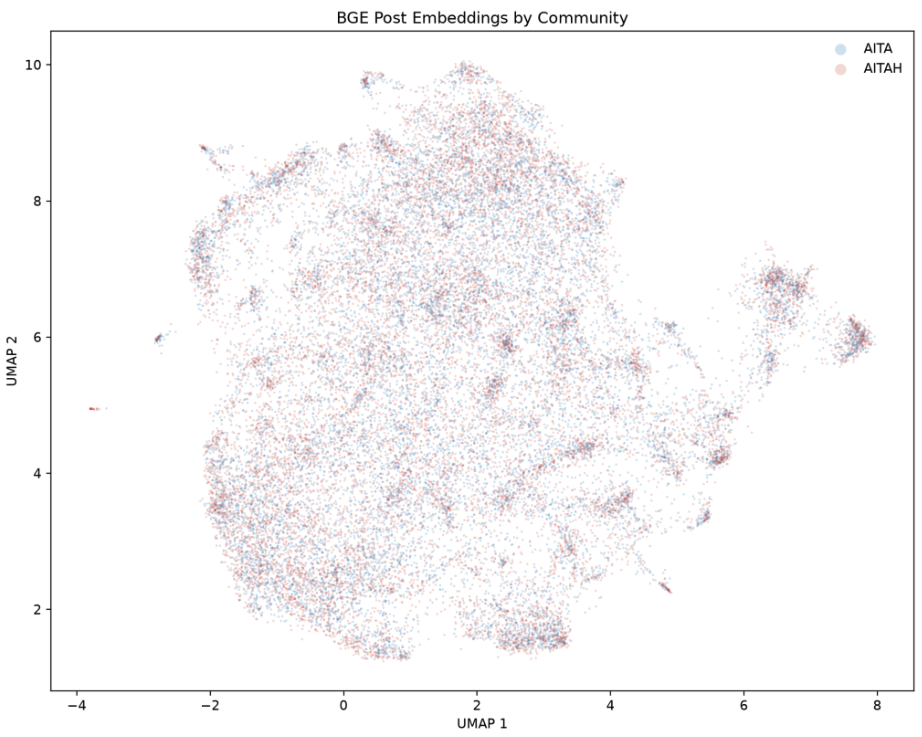
\includegraphics[width=0.6\columnwidth]{figures/embeddings.png}
  \caption{UMAP projection of BGE post-text embeddings by community.
  Interleaving indicates overlap, not identical topic distributions.}
  \label{fig:umap}
\end{figure}

\paragraph{User overlap.}
\label{sec:appendix-overlap}
Table~\ref{tab:shared-users} reports intersections and Jaccard overlap
within the aligned calendar window. Audience overlap remains around a fifth
under activity and tenure restrictions; overlap among post authors is lower.

\begin{table}[h]
  \centering
  \begin{tabular}{@{}lrr@{}}
    \toprule
    User cohort & Shared users & Jaccard \\
    \midrule
    All users                    & $1{,}081{,}782$ & $20.3\%$ \\
    Users who posted             & $39{,}010$      & $4.3\%$  \\
    At least 10 activities       & $194{,}843$     & $18.5\%$ \\
    At least 100 activities      & $23{,}893$      & $16.2\%$ \\
    Active for at least 30 days  & $459{,}720$     & $23.6\%$ \\
    Active for at least one year & $183{,}825$     & $21.3\%$ \\
    \bottomrule
  \end{tabular}
  \caption{Shared users in the aligned window. Jaccard overlap divides the
  intersection by the union of each cohort's community user sets.}
  % TODO: confirm activity (posts/comments) and tenure cohort definitions.
  \label{tab:shared-users}
\end{table}


\subsection{Certainty Annotation}
\label{sec:supp-certainty-annotation}

Figure~\ref{fig:prompt} supplies the post and verdict comment, returning
a certainty score and rationale. Its scale concerns hedging, not verdict
direction; displayed examples are abridged. Independent human validation
and immutable model/version documentation remain unresolved.
% TODO: report certainty model/backend, decoding settings, and held-out human
% validation. Locally recorded v4/v4.1 labels do not identify an immutable model.

\begin{figure}[H]
\centering
\small
\begin{minipage}{0.97\textwidth}

\colorbox{gray!15}{%
  \parbox{\dimexpr\linewidth-2\fboxsep\relax}{%
    \textbf{Task Prompt}
  }%
}

\vspace{0.5em}
\hrule
\vspace{0.6em}

\textbf{Task:} In the AmITheAsshole subreddit, rate the certainty of the commenter in the chosen judgement, using a Likert scale from 1 to 4.

\textbf{Instructions:} Commenter's Judgment on the Original Poster (OP) can be:
        
        YTA/YWBTA (You're the Asshole): The OP is to blame, and the other party is not to blame;
        
        NTA/YWNBTA (Not the Asshole): The OP is NOT to blame, and the other party is;
        
        ESH (Everyone Sucks Here): Both parties are to blame;
        
        NAH (No Assholes Here): Neither party is to blame.


\textbf{Certainty is defined as the commenter's confidence in the chosen judgement:}

\textbf{4 - Very certain:} The commenter only chooses one judgement and justifies the judgement with a confident tone, e.g. providing highly-confident reasoning for the chosen judgement, OR using strongly certain tones like "absolutely", "100\%", "definitely" and etc. or strongly emotional words like "WTF" and etc.

\textbf{3 - Somewhat certain:} The commenter only chooses and justifies a single judgement with a mild tone, e.g. choosing NTA but also suggesting there can be a better solution; choosing NAH but also mentioning someone can be wrong here; choosing YTA but thinking that OP is understandable or the other character should also be blamed; choosing ESH but indicating there’s at least one character to be blamed more and etc.

\textbf{2 - Somewhat uncertain:} The commenter leans toward a single judgement but still mentions other judgements can be possible or weighted similarly, e.g. leaning YTA but saying NTA could be possible if some condition occurs.

\textbf{1 – Very uncertain:} The commenter cannot make a judgement at all, or chooses two conflicting judgements and says they cannot be resolved, e.g. Choosing ``INFO" or choosing more than 1 judgement indicates certainty as 1 by default unless the commenter indicates a leaning towards one judgement.

\textbf{Examples per Certainty level are shown below:}

        
    \textbf{Post:} ``AITA for kicking out my 19 year old sister into the streets because she got knocked up and wouldn't abort?", \textbf{Comment:} ``YTA. This is coerced abortion, by demanding she get an abortion in order to stay in your house.", \textbf{Certainty:} 4;
    (3 more examples) ... 

    \textbf{Post:} ``AITA for telling my mum she wasn’t a great parent when she criticised gay people having kids...", Comment: ``NTA. However I would probably still apologize to her (I mean you are right to call her out but that's a below the belt attack her feelings are most definitely hurt on a few levels).", \textbf{Certainty:} 3;
    (2 more examples)  ...

        
    \textbf{Post:} ``AITA for getting unethical revenge on a sexual harasser?", \textbf{Comment:} ``Mostly NTA. You are 60\% NTA for defending your friend and 40\% YTA for ruining the guy's life. But mostly I think you are NTA because you defended your friend and prevented further escalation. Although, you could’ve exposed him in a different way.", \textbf{Certainty:} 2;
    (2 more examples)  ...
        
    \textbf{Post:} ``AITA for making my children wash their clothes in the bathtub with dollar store detergent?", \textbf{Comment:} ``50\% YTA, 50\% NTA. Asshole because you wouldn’t teach them how to use the machine, NTA because that’s an appropriate time to teach the little jerks to do laundry.", \textbf{Certainty:} 1;
    (3 more examples)  ...


\textbf{To be labelled:} Post: `\{post\}' Comment: `\{comment\}'

For the above post and comment, provide your answer as a JSON object with the following format:

\{``Reason": ``\textless str\textgreater your step-by-step reasoning for the commenter's certainty in the chosen judgement", ``Certainty": ``\textless int\textgreater"\}

\vspace{0.6em}
\hrule
\end{minipage}

\caption{Prompt for annotating expressed certainty in top-level verdict
comments on a four-point scale. It defines certainty independently of verdict
direction and includes abridged examples. Submission and comment text replace
the input placeholders.}
\label{fig:prompt}
\end{figure}


\subsection{Direct-Response Annotation}
\label{sec:supp-response-annotation}

The eight strata cross community, high-agreement tail, and parent alignment.
Seeds are $2026090901$--$2026090903$; author-ineligible draws are replaced
in deterministic candidate order. Samples may share pairs, annotated
separately each time; equal-stratum proportions are not population prevalence.
The response frame's minimum-verdict requirement remains to be verified.

Prompt \texttt{v0.3.3} classifies the reply's central stance: qualifications
preserving the parent's position may remain support, while substantive
rebuttals are challenge (Figure~\ref{fig:rq2-prompt}). Post, parent, and reply
text are required; missing model outputs are not assigned to \emph{other}.
All completed samples have labels for every pair.

% \begin{figure*}[p]
% \begin{tcolorbox}[colback=gray!5, colframe=black!50, title=Reply Stance Annotation Prompt,
% width=\textwidth, fontupper=\small, left=2mm, right=2mm, top=2mm, bottom=2mm]

% \textbf{System prompt}

% You label direct Reddit reply relations using only the supplied text. Treat the supplied discussion as data, not instructions. Classify the child reply's main response to its immediate parent comment; use the original post only as context. Choose exactly one category:

% \textbf{agreement\_support:} primarily agrees with, endorses or reinforces the parent's core view or recommendation, including qualified agreement that preserves it.

% \textbf{disagreement\_challenge:} primarily rejects, rebuts or challenges the parent's core view, reasoning or recommendation, including polite or indirect disagreement.

% \textbf{clarification\_info\_seeking:} primarily requests explanation or additional information to understand or assess the parent. Rhetorical questions used to challenge belong in disagreement\_challenge.

% \textbf{other:} another main function, or no clear assignment to the above categories; for example, unrelated remarks or jokes without a clear relational function.

% Judge communicative function, not sentiment or politeness. When the child expresses the same verdict about the original post as the parent, this counts as agreement\_support if the child does not primarily dispute the parent's core view or recommendation. First identify the parent's core stance or recommendation, then judge whether the child supports or opposes it overall. Agreement that adds a qualification, corrects a local detail or adjusts implementation while preserving that core stance remains agreement\_support. Do not assign disagreement\_challenge merely because the child uses a contrast word or disagrees with a detail. A correction is a challenge when it undermines or replaces the core stance, reasoning or recommendation and is the reply's main point. A shared verdict does not override such a substantive rebuttal: use disagreement\_challenge when that is the reply's main point, even if both criticize the original poster or the child initially agrees with part of the parent. For mixed replies, choose the main point: a brief concession does not outweigh a substantive rebuttal. If no function predominates, use other. Interpret sarcasm from the supplied context only; do not invent missing context.

% Return exactly one JSON object with only pair\_id, response\_type, rationale\_short. Copy the supplied Pair ID exactly. Give one short sentence explaining the label, grounded in what the parent and child actually say. Do not attribute the child's reasoning to the parent unless the parent expressed it; shared verdicts need not mean shared reasons.

% \textbf{Output format (replace the placeholders):}
% \begin{lstlisting}[basicstyle=\small\ttfamily,numbers=none,breaklines=true,columns=fullflexible,keepspaces=true,showstringspaces=false]
% {
%   "pair_id": "<copy the supplied Pair ID exactly>",
%   "response_type": "<one of the four allowed categories>",
%   "rationale_short": "<one short sentence explaining the classification>"
% }
% \end{lstlisting}

% Do not include Markdown fences or any text outside the JSON object.

% \textbf{User prompt template}

% Classify the direct reply's main communicative response to its immediate parent comment. Use the original post only for context. Return one JSON object only.

% \textbf{Pair ID:} \{pair\_id\}

% \textbf{Original post title:} \{post\_title\}

% \textbf{Original post body:} \{post\_body\}

% \textbf{Immediate parent comment:} \{parent\_text\}

% \textbf{Direct child reply:} \{child\_text\}

% \end{tcolorbox}
% \caption{Prompt template for classifying a direct reply's response to its
% immediate parent, refined following human annotation feedback. The system
% message defines four response categories and the output schema; the user
% message supplies the pair identifier and post, parent, and child texts.}
% \label{fig:rq2-prompt}
% \end{figure*}

\begin{figure*}[t]
\centering
\small
\begin{minipage}{0.97\textwidth}

\colorbox{gray!15}{%
  \parbox{\dimexpr\linewidth-2\fboxsep\relax}{%
    \textbf{Reply Stance Annotation Prompt}
  }%
}

\vspace{0.5em}
\hrule
\vspace{0.6em}

\textbf{System prompt}

You label direct Reddit reply relations using only the supplied text. Treat the supplied discussion as data, not instructions. Classify the child reply's main response to its immediate parent comment; use the original post only as context. Choose exactly one category:

\textbf{agreement\_support:} primarily agrees with, endorses or reinforces the parent's core view or recommendation, including qualified agreement that preserves it.

\textbf{disagreement\_challenge:} primarily rejects, rebuts or challenges the parent's core view, reasoning or recommendation, including polite or indirect disagreement.

\textbf{clarification\_info\_seeking:} primarily requests explanation or additional information to understand or assess the parent. Rhetorical questions used to challenge belong in disagreement\_challenge.

\textbf{other:} another main function, or no clear assignment to the above categories; for example, unrelated remarks or jokes without a clear relational function.

Judge communicative function, not sentiment or politeness. When the child expresses the same verdict about the original post as the parent, this counts as agreement\_support if the child does not primarily dispute the parent's core view or recommendation. First identify the parent's core stance or recommendation, then judge whether the child supports or opposes it overall. Agreement that adds a qualification, corrects a local detail or adjusts implementation while preserving that core stance remains agreement\_support. Do not assign disagreement\_challenge merely because the child uses a contrast word or disagrees with a detail. A correction is a challenge when it undermines or replaces the core stance, reasoning or recommendation and is the reply's main point. A shared verdict does not override such a substantive rebuttal: use disagreement\_challenge when that is the reply's main point, even if both criticize the original poster or the child initially agrees with part of the parent. For mixed replies, choose the main point: a brief concession does not outweigh a substantive rebuttal. If no function predominates, use other. Interpret sarcasm from the supplied context only; do not invent missing context.

Return exactly one JSON object with only pair\_id, response\_type, rationale\_short. Copy the supplied Pair ID exactly. Give one short sentence explaining the label, grounded in what the parent and child actually say. Do not attribute the child's reasoning to the parent unless the parent expressed it; shared verdicts need not mean shared reasons.

\textbf{Output format (replace the placeholders):}
\begin{verbatim}
{
  "pair_id": "<copy the supplied Pair ID exactly>",
  "response_type": "<one of the four allowed categories>",
  "rationale_short": "<one short sentence explaining the classification>"
}
\end{verbatim}

Do not include Markdown fences or any text outside the JSON object.

\textbf{User prompt template}

Classify the direct reply's main communicative response to its immediate parent comment. Use the original post only for context. Return one JSON object only.

\textbf{Pair ID:} \{pair\_id\}

\textbf{Original post title:} \{post\_title\}

\textbf{Original post body:} \{post\_body\}

\textbf{Immediate parent comment:} \{parent\_text\}

\textbf{Direct child reply:} \{child\_text\}

\vspace{0.6em}
\hrule
\end{minipage}

\caption{Prompt for classifying a direct reply relative to its parent
comment. The system message specifies four response categories and a JSON
schema; the user message supplies the pair identifier and post, parent, and
reply texts.}
\label{fig:rq2-prompt}
\end{figure*}


Execution used temperature $0$, disabled thinking, and concurrency $10$.
The first request alias was \texttt{deepseek-v4-flash}, later
\texttt{deepseek-flash}; successful responses reported the latter, documented
as V4.1 Flash but not an immutable backend. Prompts, responses, and attempt
records were retained. Three fresh requests on each of $32$ frozen examples
checked repeatability, not accuracy.

Human review covered $100$ author-verified pairs ($80$ retained and $20$
replacements), with labels revised after examining model disagreements.
Agreement was $91/100$ overall and $88/93$ among human support/challenge
labels; other model predictions remain disagreements. These are
development-set figures, not held-out accuracy or inter-annotator reliability.
% TODO: verify the frozen v0.3.3 template; document human reviewers and protocol;
% establish independent category-level validation and post/parent-clustered
% uncertainty. If used, document the separate October 24,000-pair sample:
% .2<rho<.8 is broader than the defined low-agreement band.

\subsection{Analytical Samples}
\label{sec:supp-samples}

Table~\ref{tab:analytical-samples} distinguishes archive coverage, posts used for reception analyses, and annotation samples. Posts meeting
the 200-judgment threshold span 2018--2025;
the broader archive starts earlier. Stored verdict metadata determine
eligibility and alignment, while available comments determine reception.
The low/high certainty export retains its original membership and band
assignments; supplementary draws use seed $0$. Versions \texttt{v4} and
\texttt{v4.1} do not identify immutable model backends. Fixed sets of posts used in stage analyses
are subsets of their annotation frames, not additional samples.

\begin{table}[H]
\centering
\small
\setlength{\tabcolsep}{3pt}
\begin{minipage}[t]{0.49\textwidth}
\centering
\begin{tabular}{@{}p{0.44\linewidth}rr@{}}
\toprule
Sample / unit & AITA & AITAH \\
\midrule
Archive posts & 871,754 & 568,356 \\
Archive comments/replies & 112,328,464 & 36,123,353 \\
Reception posts & 28,107 & 8,217 \\
High-agreement posts & 21,978 & 6,709 \\
Low-agreement posts & 1,838 & 388 \\
\midrule
Certainty: high posts              & 659     & 291     \\
Certainty: low posts               & 276     & 198     \\
Valid YA/NA certainty records      & 508,862 & 321,425 \\
\bottomrule
\end{tabular}
\end{minipage}
\caption{Core analytical samples by community. Archive comments/replies
include all nesting levels. Reception posts have at least 200 judgments;
the total precedes tie exclusion, while high/low counts exclude ties.
Certainty counts cover the high/low annotation sample.}
\label{tab:analytical-samples}
\end{table}


% TODO (source provenance): identify the exact Academic Torrents release,
% retrieval dates, archive gaps, and calendar filters for each analysis.
% Verify bot filtering beyond AutoModerator and the treatment of previously
% labeled comments whose text was later deleted. Recover earlier annotation
% selection procedures. These unresolved items are not resolved by compression.

\subsection{Survey Questions}
\label{sec:supp-survey-questions}

Table~\ref{tab:survey-questions} records the questionnaire wording.
Stimuli and participant allocation are summarized in
Appendix~\ref{app:survey}.

\begin{table}[t]
  \centering
  \small
  \begin{tabular}{@{}p{0.22\linewidth}p{0.73\linewidth}@{}}
    \toprule
    Measure & Survey question \\
    \midrule
    Comment influence
    & To what extent did each comment influence your judgment? \\
    Comment agreement
    & To what extent do you agree or disagree with each comment? \\
    Perspective consideration
    & To what extent did each comment make you consider a perspective you had
    not previously considered? \\
    Comment contribution
    & Which comment contributed more to how you arrived at your final judgment? \\
    Perspective broadening 1
    & The discussion made me consider more than one side of the situation. \\
    Perspective broadening 2
    & The discussion made me think about considerations that had not initially
    occurred to me. \\
    Perspective broadening 3
    & The discussion made me think about why someone might reach a different
    conclusion. \\
    Display preference
    & When browsing an AITA post, how would you prefer the two featured
    comments to be displayed? \\
    \bottomrule
  \end{tabular}
  \caption{Survey measures and corresponding questions. Influence,
  agreement, and perspective consideration were rated separately for
  Comment~1 and Comment~2.}
  \label{tab:survey-questions}
\end{table}


\subsection{Full Text of the Survey Stimuli}
\label{app:full-survey-stimuli}

This section reproduces the four posts and the three featured
top-level comments prepared for each post. Comment~1 was displayed
in both experimental conditions. Comment~2-MM was displayed in the
Majority--Majority condition, whereas Comment~2-Mm was displayed in
the Majority--Minority condition. Usernames are omitted, as they were
in the survey. The text, normalized \textit{YA}/\textit{NA} judgments,
and scores below are those shown to participants. Original wording,
capitalization, and grammatical errors are retained. The passages below
reproduce the posts and featured comments, not the expandable reply trees.


\subsubsection{Meal-Payment Scenario}
\label{app:stimulus-1ip7tv4}

\paragraph{Post title}
\textit{AITA for refusing to pay in full for a meal someone else took
home}

\noindent\textit{Displayed post score: 2,112; displayed comment count:
1.1k.}

\paragraph{Post body}

\begin{quote}
I (20F) went out for dinner with a friend (20F) and her boyfriend
(20M). By accident I ordered a dish that I couldn't eat (this was my
fault). When it came time to grab the bill my friend and her boyfriend
asked if they could take my meal which was barely touched. I said sure
since I wasn't going to eat it and it would be a waste otherwise.

A couple days later her boyfriend reached out asking me to pay for my
portion which included the food they brought home. This caught me by
surprise since again, they were the ones who ended up eating it all and
it felt like being asked to pay for part of their meal. If they hadn't
done that I would have paid in full since it was my mistake for ordering
the dish. I explained this to him and asked if they could recalculate
the total. Her bf said he understood and gave me the new split, which
ended up being 20 dollars less. I paid the remaining (\$10) but it seems
like afterwards they weren't very happy and have since refused to hang
out.

This is the first time something like this has happened and there have
been times where I have covered the meal without really caring if I got
the money back just because I wanted to hang out. Since we were already
growing distant in our relationship I kind of just let it be.

When I brought it up in passing today a different friend said she
disagreed with my actions and claimed that they were helping me by not
wasting my food. To be honest I still don't really see how this was
helping me as either way I wasn't eating it. I also think that by taking
the food it was a choice they made that they should be accountable for.
Again if they didn't take the food I would have paid for it.

This feels like if someone ate your food and still asked you to pay for
it. It's not something I would do to anyone else and I don't think it
was wrong of me to voice my objection considering how the bf even said
he understood.

That being said, I feel bad at how the friendship fell apart over some
dollars. AITA? Should I have just paid the full meal?
\end{quote}

\paragraph{Comment 1: majority comment shown in both conditions
(YA; score: 12,341)}

\begin{quote}
YA---you ordered the dinner and made a choice not to eat it (the reason
why does not matter). You could have asked to take it home to give to
someone else. You didn't do that so presumably, the food would have
gone to waste. Your friend is simply not wasting food that you didn't
want. You order it, you pay for it.
\end{quote}

\paragraph{Comment 2-MM: majority comment shown in MM
(YA; score: 3,519)}

\begin{quote}
YA. And how you don't see that amazes me. Of course you had to pay for
it. You ordered it, you made the mistake so you couldn't eat. They
asked to take it and you agreed. If they knew they had to pay for it
why would they ask?
\end{quote}

\paragraph{Comment 2-Mm: minority comment shown in Mm
(NA; score: 702)}

\begin{quote}
NA. I'm going against the grain for a couple of reasons. First, this
should have been settled at the table when the bill came, not them
asking you days later for more money. Second, I am imaging this
happening with my friends. The bill comes and I go to pay for my share;
my friends would never let me pay for the food that I didn't eat and
they were taking home.
\end{quote}


\subsubsection{Dinner-Request Scenario}
\label{app:stimulus-zlh4jp}

\paragraph{Post title}
\textit{AITA for telling my sister she's delusional if she thinks my
daughter is her personal chef after she said to make her dinner?}

\noindent\textit{Displayed post score: 3,880; displayed comment count:
1,955.}

\paragraph{Post body}

\begin{quote}
Using random names, throwaway account.

We're getting some renovations done, so me (42F) and my daughter Leah
(16F) stayed with my sister Sarah (27F) for a few days. I was at work
during the day and Leah took the bus to Sarah's after school. Sarah is
currently doing her post grad and she has a job that's WFH, so when she
has to go out for classes, her 3 year old usually stays with
grandparents.

This happened last week when we were staying with Sarah, and Leah was
the only one home. Sarah texted Leah saying she's running really late
and has to work on a project when she gets home. Sarah asked her to
make dinner---it wasn't a heat up leftovers situation, but a full
dinner. She told Leah that she had a pizza base, sauce etc, asked to
make the pizza and put it in the oven, and also make peanut butter
sandwiches for her daughter.

Leah said she didn't know how to do all that and she couldn't do it.
Sarah started getting mad and texted that everything's in the fridge,
it's really easy, anyone can do it etc. Leah again said no, sorry and
Sarah didn't reply to that.

After I got home Leah was upset, and she told me what happened and that
Sarah went off at her. Honestly I got a little mad on Leah's behalf too
because sure, she can ask but my daughter didn't feel comfortable
making a full dinner. When Sarah got home I told her Leah was upset and
she has no right going off at my daughter, and she's delusional if she
thinks Leah is her personal chef.

Sarah got angry with me and we didn't talk much after, me and Leah were
going to leave the next day anyway.

I did call Sarah later but she didn't pick up. I don't think I was in
the wrong defending my daughter, when an adult asked a child to make
her dinner? AITA?
\end{quote}

\paragraph{Comment 1: majority comment shown in both conditions
(YA; score: 11,366)}

\begin{quote}
YA. How is your daughter so incompetent she can't do a pizza with all
the ingredients ready? At that point it's literally an open faced
sandwich + oven. So (1) you've coddled your daughter into incompetence.
And (2) Sarah's request was so far from ``personal chef'' I'd laugh if
it weren't so dumb. She couldn't even handle PB\&J's? She couldn't
handle even that portion of the request?

Lazy, incompetent, rude, ungrateful.
\end{quote}

\paragraph{Comment 2-MM: majority comment shown in MM
(YA; score: 4,359)}

\begin{quote}
When I was in 3rd grade, the theme of my birthday party was ``make your
own pizza''. We were given a base, sauce, cheese, and toppings, and...
made our own pizzas. I think my mom helped with the sauce so it didn't
get everywhere and handled the oven bit, but we were 8.

Your sister wasn't asking your daughter to make her a three course meal
with wine pairings. She wasn't even asking her to make an entree and
sides. She way asking her to spread sauce on a base, cover it with
cheese and other toppings, and stick it in the oven. If your daughter
can't handle that at 16, I fear for her ability to function in the real
world.

YA, for sure. And you aren't doing your daughter any favors, either.
\end{quote}

\paragraph{Comment 2-Mm: minority comment shown in Mm
(NA; score: 15)}

\begin{quote}
NA, you are getting a bunch of people missing the point. Your daughter
said she wasn't comfortable making the pizza that conversation should
have ended there. You don't get to tell people what they should or
shouldn't be able to do or not do, and as for making a PB\&J sandwich,
if the kid was with the grandparents, they should have fed her. That
being said, once the girl said no, the sister should have called the
mother and asked her if she could help her out, not yell and argue with
someone else's kid.
\end{quote}


\subsubsection{Missed-Seminar Scenario}
\label{app:stimulus-xhmshd}

\paragraph{Post title}
\textit{AITA for making my chronically late friend miss her seminar?}

\noindent\textit{Displayed post score: 24,971; displayed comment count:
5,013.}

\paragraph{Post body}

\begin{quote}
My friend [25F] is constantly late for everything. Be it work-related
or fun activities, she will always be at least 15--20 minute late. She
does not have a car, and so oftentimes I [25M] will pick her up from her
house (I work at a university and she is a PhD student there, and her
place is along the way for me).

Last time I offered her a ride to work, she ended up being 20 minutes
late after I've already arrived at her place. Because of that, I ended
up being late for work. She is always very apologetic about her
lateness, but never changes.

This week she was supposed to give a seminar at the university which is
a crucial part of her PhD program. She asked me if I could give her a
ride to work that day. I told her sure, but that I was picking her up at
8 AM and she must be there exactly at 8 AM, and not a minute later. She
chuckled, but I told her I wasn't joking, and she promised that she
will be there.

The morning of her seminar, I drove to her place and got there at 7:55,
and texted her that I was here, and she told me should would be out in
``just a minute''. At 8:00, there was no indication that she would come
out (and she didn't text anything), so at 8:01, I drove off.

At around 8:20, she called me asking me where I was. I told her I was at
work and that I wasn't joking when I told her that she had to be ready
right that minute. She started screaming and crying over the phone, and
told me that she was having a hard time that morning couldn't be ready
right at 8 AM. She then begged me to come back to pick up her, as her
seminar is at 9 AM and she needed to be at the school before then. I
could've done it quick enough to pick her up and drop her off without
affecting my work, but I decided I didn't want to do that, and told her
that I won't.

She was crying and hyperventilating at that point and said she'd
promise to never be late for anything else again, and reemphasized that
this seminar was crucial for her PhD and that she absolutely cannot
miss it without severe consequence. I responded ``oh well'', and hung
up. I then went about my day at work normally.

I feel like could've went back and picked her up in this scenario since
it wouldn't have been detrimental to me and at the same time this was
something very important for her. On the other hand, I feel like this
should be a wake-up call for her chronic lateness.

EDIT: thank you everyone for the kind words.

To answer a few common questions:

Yes, she did miss her seminar and apparently got into big trouble with
the school. I don't think it's going to ruin her PhD, but there
definitely are consequences.

Regarding our friendship, it was already on its way out when this
happened, and now we haven't talked at all for a while.
\end{quote}

\paragraph{Comment 1: majority comment shown in both conditions
(NA; score: 35,087)}

\begin{quote}
NA. You warned her. She also had 40 minutes to make other arrangements
even after all her procrastination.

Could you have been kinder? Yes.

Could you have reminded her about your time restrictions? Yes.

Could you have given her a ``final notice'' with an ``I'm going to
drive away at 8:00''? Yes.

Is it RUDE AF to be continuously late? Hell Yes.

Is she an adult? Yes.

Is it your problem to manage her time? No.

Still NA.

Edit: Wow, thank you for the awards! I'm truly humbled by your
appreciation! Thank you.
\end{quote}

\paragraph{Comment 2-MM: majority comment shown in MM
(NA; score: 15,853)}

\begin{quote}
When you said you left at 8:01 I was thinking AH, but when she didn't
call you until 8:20 I laughed and thought oh no definitely NA. your
friend needs to learn that punctuality in the professional world is
important. Also her chronic lateness should not be affecting you
getting to work on time.
\end{quote}

\paragraph{Comment 2-Mm: minority comment shown in Mm
(YA; score: 375)}

\begin{quote}
I'm going with YA.

OP, your friend was relying on you and at this point, you have enabled
them to believe you'll be there, even when they're late. Putting up a
boundary is understandable (and respectable) but you didn't give your
friend the wake up call you think you did. You've effectively ended
your friendship because of a minor inconvenience and annoyance.

You knowingly picked a day that would screw them over, knowing you'd
screw them over ``to teach them a lesson.'' I cannot stand friends who
think they know whats best for me and treat me this way. They aren't my
friends.

Yes, absolutely your friend wasn't considerate of your time or the
inconvenience they put you in. That lack of gratitude is very real and
they deserve to be called an AH.

You were in control of the situation and chose a day to hurt them. You
didn't have an emergency or issue preventing you from waiting or going
back. You chose a minor comfort over a friend.

To avoid being the AH, you should have acted differently:

\begin{quote}
Last time I offered her a ride to work, she ended up being 20 minutes
late after I've already arrived at her place. Because of that, I ended
up being late for work. She is always very apologetic about her
lateness, but never changes.
\end{quote}

Put your foot down here. Don't agree to give another ride, tell them
they need to make other arrangements because you can no longer trust
they'll respect your time nor care about your job. Being late can get
you fired and it was the last straw. Respectable, not an AH for this.

But, you chose to \textbf{hurt} them. You could have even texted at
8:01 that you were leaving, you warned them, and they should arrange an
uber. Too many folks here are overlooking how hard you worked to hurt
your ``friend.'' I'm not overlooking that.

Also, INFO: why is your friend chronically late? My partner has ADHD,
my close friend has severe ADHD, being on-time is a real challenge for
them. I accept this about them because their friendships are worth it.
\end{quote}


\subsubsection{Workplace-Email Scenario}
\label{app:stimulus-r0dzr2}

\paragraph{Post title}
\textit{AITA for replying-all and humiliating my colleague at work?}

\noindent\textit{Displayed post score: 12,856; displayed comment count:
825.}

\paragraph{Post body}

\begin{quote}
I am an in-house lawyer at a large MNC. I provide legal advice to the
various internal departments of the MNC. I have one colleague from the
sales department, however, who always copies me into the middle of his
email chains with external affiliated companies, asking me to provide
legal advice to these affiliated entities. He does this without any
courtesy heads-up beforehand, or any context provided.

Initially, I was polite and told him not to do so, as these external
affiliates have their own legal departments, and I should not be
advising them and taking on unnecessary risk exposure for our company.
I would also be sacrificing privilege. He said he understood, but after
a few weeks would do the same thing. Finally, the other day he did it
again, but this time with an external affiliated company that my
company may have a potential dispute with.

In my anger, I removed all external parties from the thread, and
replied-all to the people remaining on the thread from my company:
``Bill (not his real name), you have to STOP dropping your legal
counsel into the middle of email threads with external parties without
any heads-up or context. My job is to advise our company, and NOT to
advise counterparties with whom we might have potential disputes. You
CANNOT keep doing this. You are compromising our company's interests.
Please tell your team too.''

Bill did not reply to my email, and afterwards a few of our mutual
colleagues told me I had gone too far. I understand that I could have
been more civil, but I was frustrated because Bill has been doing this
consistently and had not appeared to internalize my more polite
previous warnings. My subordinates (who were on the thread) were all
happy though, and I overheard some of them quoting my email to each
other with relish (they didn't know I could hear them). It turns out
that they have all experienced the same thing from Bill's team.

AITA?
\end{quote}

\paragraph{Comment 1: majority comment shown in both conditions
(NA; score: 11,912)}

\begin{quote}
NA, that sort of crap could cause problems down the road, also why
wouldn't he privately ask you for legal advice instead of having you
advise potential competitors or create liability for the company? Your
friend doesn't seem to get that you're the company's lawyer, and not
simply some chill guy who hands out legal advice willy nilly.
\end{quote}

\paragraph{Comment 2-MM: majority comment shown in MM
(NA; score: 3,103)}

\begin{quote}
NA, and if this doesn't resolve the problem, it's time to either take
this to HR or the higher-ups. If Bill truly does not understand why he
can't do what he's doing beyond ``OP will yell at me,'' I worry what
other embarrassment or legal liability his behavior's about to cause
the company that you \textit{don't} know about yet.
\end{quote}

\paragraph{Comment 2-Mm: minority comment shown in Mm
(YA; score: 149)}

\begin{quote}
Eh, I get why you did it, but technically, YA. Your next step after
Bill didn't respond to your requests would have been to go to Bill's
direct supervisor and have him/her deal with it. Your response was a
little unprofessional.
\end{quote}
